
% this file is called up by thesis.tex
% content in this file will be fed into the main document
%: ----------------------- introduction file header -----------------------
\chapter{Introduction}

% the code below specifies where the figures are stored
\ifpdf
    \graphicspath{{1_introduction/figures/PNG/}{1_introduction/figures/PDF/}{1_introduction/figures/}}
\else
    \graphicspath{{1_introduction/figures/EPS/}{1_introduction/figures/}}
\fi

% ----------------------------------------------------------------------
%: ----------------------- introduction content ----------------------- 
% ----------------------------------------------------------------------



%: ----------------------- HELP: latex document organisation
% the commands below help you to subdivide and organise your thesis
%    \chapter{}       = level 1, top level
%    \section{}       = level 2
%    \subsection{}    = level 3
%    \subsubsection{} = level 4
% note that everything after the percentage sign is hidden from output



\section{Context} \label{section:intro.contex}
The Low Frequency Array(LOFAR) telescope\footnote{\url{http://www.lofar.org/}} consists of 51 stations across Europe, and a typical LOFAR observation has the size of 100 TB which can be reduced to 16 TB after frequency averaging\cite{Spreeuw2019}.
Collectively, there are over 5 PB of data to be stored each year\cite{Start2020}. 
In the case that the data-collecting speed exceeds the processing capability, the data will be stored and archived first, and then processed at the request of the researchers on astronomy, physics and computer science. 
The pipeline is divided into multiple steps, and in this thesis, we focus on the calibration which is available to reduce the noise of observation. 
The Netherlands eScience Center\footnote{\url{https://www.esciencecenter.nl/}} has developed solutions for calibrating imaged observation collected by LOFAR. As one of the implementation for image calibration, Sky map is based on direction independent calibration. 
SAGECaL is designed and implemented to calibrate the observation by a given sky map\cite{Kazemi2011}.

Using the given pre-processed observation data, sky model and parameters for computation i.e. number of iterations, the input data can be processed in parallel, which is, however still a computational intensive application. 
Currently, GPU, MPI\footnote{\url{https://github.com/nlesc-dirac/sagecal}}, and Spark\footnote{\url{https://github.com/nlesc-dirac/sagecal-on-spark}} versions are developed by eScience Center to speed up the data processing, which all have achieved high acceleration compared with the naive uni-node version.
The GPU version provides great acceleration. 
Though the computation capability of single node is expanded, it is still vertical scaling\ref{Vscaling}.
 On the other hand, MPI and Spark implementations can be considered as horizontal scaling\ref{Hscaling}, and the entire computational power increases via adding more resources. 
 Of course, these two horizontal scaling approaches are also able to add GPU to make worker nodes more powerful. 
 However, all these three solutions show their own limitations.

LOAFR is one of the use cases of ASTRON\footnote{\url{https://www.astron.nl/}}.
ASTRON builds its own clusters to meet the demands for data processing. 
Therefore, the resource utilization of its infrastructures is also essential. 
The current implementations focus on the efficiency and utilization of assigned resources.  
In theory, MPI and Spark solutions may lead to a potential waste of resources to the whole cluster, which ASTRON expects to minimize.
Fig. \ref{fig:sparkUti} shows an example of computing resource waist of the spark implementation when the required computation resources decrease, Spark does not release idle resources(compute nodes). 
On the other hand, a pure batch-job system may get easily into a special situation that a big job is waiting for the resource while idle resources cannot fulfill the requirement, an example is shown in Fig. \ref{fig:MPIUti}. 
The figure shows the possible resource waste represented by the blank area.



\begin{figure}
    \centering
    \begin{minipage}{.5\textwidth}
      \centering
      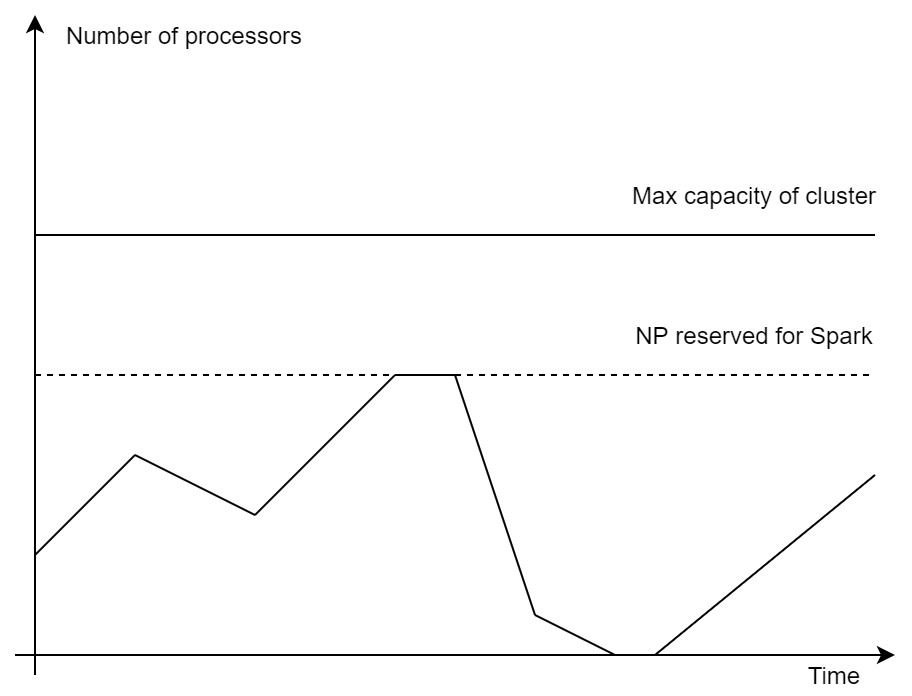
\includegraphics[width=0.9\linewidth]{1_introduction/figures/spark_NP.jpg}
      \caption[SparkUti]{{\small\textbf{Resource utilization by Spark} - Spark occupies fixed resources}}
      \label{fig:sparkUti}
    \end{minipage}%
    \begin{minipage}{.5\textwidth}
      \centering
      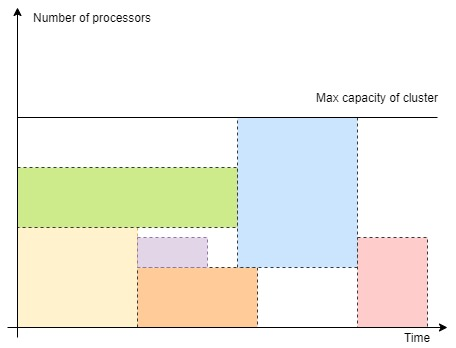
\includegraphics[width=0.9\linewidth]{1_introduction/figures/MPI_batch.jpg}
      \caption[MPIUti]{{\small\textbf{Resource utilization by MPI} - Too large jobs make resource waste}}
      \label{fig:MPIUti}
    \end{minipage}
\end{figure}
The eScience center has developed Xenon\footnote{\url{https://xenon-middleware.github.io/xenon/}} a middleware which aims to provide uniformed and simple interface to enable application program to access both computation and storage resources.
Using Xenon interfaces, it is possible to submit jobs, and access the status of jobs and the cluster without parsing the output of control commands from resource manager. 
Besides, the computer system group of VU Amsterdam has developed Ibis\footnote{\url{https://www.cs.vu.nl/ibis/}} a platform  for efficient distributed computing. 
The Ibis Portability Layer, a sub-module of Ibis, enables computing entities to communicate with each other in a reliable cluster environment.

In this work, we use both Xenon and Ibis to manage the jobs and resource at a high level.
\section{Objective}

The mian objective of this project, is to achieve higher resource utilization of the cluster. 
At the same time, as a secondary objective, we aim to accelerate the calibration processing. 
In theory, higher resource utilization may lead to more active computation resources involved. 
To achieve these goals, we develop a system which reduces the time to wait for large distributed jobs.
\section{Research Question}
The overall research question is how to design and implement a distributed resource management system which can reduce the waste of resources.

\section{Research Method}
In this research, firstly, we briefly describe the common used resource management techniques in HPC clusters and analyse the  MPI and SPARK implementations to identify bottleneck, or limitation.
Secondly, we will implement a resource management system that is able to scale up and down the computing resources dynamically according to the application workloads,  and so that the whole cluster can achieve overall higher resource utilization. 
Finally, we will test the performance of the system by comparing the resource utilization before and after the employment of this system. 
To validate our results, we will use the LOFAR calibration pipeline(SAGECaL), and the calibration jobs can be divided well due to the features of SAGECaL.
